%%%%%%%%%%%%%%%%%%%%%%%%%%%%%%%%%%%%%%%%%%%%%%%%
% BOZZA PER TESI DI LAUREA IN LATEX
%%%%%%%%%%%%%%%%%%%%%%%%%%%%%%%%%%%%%%%%%%%%%%%%

\documentclass[12pt,titlepage]{report}
\usepackage[english,italian]{babel}
\usepackage{graphics}
\usepackage{upgreek}
\usepackage{url,amsfonts,epsfig} 
\usepackage[utf8x]{inputenc} % comando per le lettere accentate
\usepackage{ dsfont }
\usepackage{caption}
\usepackage{subcaption}
\usepackage{listings}
\usepackage{color}
\usepackage{float}
\definecolor{mygreen}{rgb}{0,0.6,0}
\definecolor{mygray}{rgb}{0.5,0.5,0.5}
\definecolor{mymauve}{rgb}{0.58,0,0.82}
\lstset{ 
	backgroundcolor=\color{white},   % choose the background color; you must add \usepackage{color} or \usepackage{xcolor}; should come as last argument
	%basicstyle=\footnotesize,        % the size of the fonts that are used for the code
	basicstyle=\tiny,
	breakatwhitespace=false,         % sets if automatic breaks should only happen at whitespace
	breaklines=true,                 % sets automatic line breaking
	captionpos=b,                    % sets the caption-position to bottom
	commentstyle=\color{mygreen},    % comment style
	deletekeywords={...},            % if you want to delete keywords from the given language
	escapeinside={\%*}{*)},          % if you want to add LaTeX within your code
	extendedchars=true,              % lets you use non-ASCII characters; for 8-bits encodings only, does not work with UTF-8
	frame=single,	                   % adds a frame around the code
	keepspaces=true,                 % keeps spaces in text, useful for keeping indentation of code (possibly needs columns=flexible)
	keywordstyle=\color{blue},       % keyword style
	language=Matlab,                 % the language of the code
	morekeywords={*,...},            % if you want to add more keywords to the set
	numbers=left,                    % where to put the line-numbers; possible values are (none, left, right)
	numbersep=5pt,                   % how far the line-numbers are from the code
	numberstyle=\tiny\color{mygray}, % the style that is used for the line-numbers
	rulecolor=\color{black},         % if not set, the frame-color may be changed on line-breaks within not-black text (e.g. comments (green here))
	showspaces=false,                % show spaces everywhere adding particular underscores; it overrides 'showstringspaces'
	showstringspaces=false,          % underline spaces within strings only
	showtabs=false,                  % show tabs within strings adding particular underscores
	stepnumber=1,                    % the step between two line-numbers. If it's 1, each line will be numbered
	stringstyle=\color{mymauve},     % string literal style
	tabsize=2,	                   % sets default tabsize to 2 spaces
	title=\lstname                   % show the filename of files included with \lstinputlisting; also try caption instead of title
}

\usepackage{amsmath}

\title{Implementazione di una\\ Echo State Network}
\author{Eleonora Di Gregorio}





\begin{document}
\pagenumbering{roman}
%%%% Opzione per interlinea 2
\baselineskip 18pt
%\maketitle

%%%%%%%%%%%%%%%%%%%%%%%%%%%%%%%%%%%%%%%%%%%%%%%%%%
\begin{titlepage}
	\begin{center}
		{{\Large{\textsc{Universit\`a di Pisa\\}}}}
	\begin{figure}[h!]
		\centering 
		
\includegraphics[width=0.3\linewidth]{immagini/Stemma_unipi.png}
	\end{figure}	
		{\bf Dipartimento di Informatica}
		%{\small{\bf FACOLT\`A DI SCIENZE MATEMATICHE, FISICHE E NATURALI\\
		%Corso di Laurea Magistrale in Matematica}}
	\end{center}
	\vspace{12mm}
	\begin{center}
		{\LARGE{\bf Implementazione di una}}\\
		\vspace{3mm}
		{\LARGE{\bf Echo State Network}}\\
		\vspace{12mm} {\large{\bf Esperienze di programmazione}}
	\end{center}
	\vspace{12mm}
	\par
	\noindent
	\begin{minipage}[t]{0.47\textwidth}
		{\large{\bf Professore:\\
				Francesco Romani\\}}
	\end{minipage}
	\hfill
	\begin{minipage}[t]{0.47\textwidth}\raggedleft
		{\large{\bf Presentata da:\\
				Eleonora Di Gregorio \\
				(520655)}}
	\end{minipage}
	\vspace{20mm}
	\begin{center}
		{\large{\bf Aprile\\%inserire il numero della sessione in cui ci si laurea
				A.A. 2017/2018 }}%inserire l'anno accademico a cui si è iscritti
	\end{center}
\end{titlepage}
%%%%%%%%%%%%%%%%%%%%%%%%%%%%%%%%%%%%%%%%%%%%%%%%%%

\tableofcontents
\listoffigures
\listoftables

\chapter{Introduzione} \label{introduzione}
\pagenumbering{arabic}

Il \textit{Reservoir Computing} (RC) \`e un metodo di grande interesse nel campo della ricerca sulle reti neurali ricorrenti (RNR), grazie alla sua semplicit\`a e alle sue buone performance su una certa variet\`a di \textit{task}. Con \textit{Reservoir Computing} ci si riferisce  ad una classe di modelli di reti neurali ricorrenti che sono caratterizzati da una parte dinamica ricorrente e una parte di output semplice. L'idea alla base del \textit{Reservoir Computing} \`e quella di prendere una rete ricorrente random di semplici nodi, ad esempio neuroni sigmoidali,chiamata appunto \textit{reservoir}. I nodi sono collegati tra loro, associando dei pesi ai collegamenti che possono essere riscalati per imporre il regime dinamico desiderato. Il \textit{reservoir} permette dunque di mappare un input in uno spazio di dimensione maggiore che nel caso di \textit{task} di classificazione pu\'o aumentare la probabilit\'a di separazione lineare tra i dati. Oltre  a questo permette anche di tenere traccia della storia degli input nel tempo, questi aspetti lo rendono ideale per molti \textit{task} interessanti nel mondo reale che richiedono elaborazione temporale e \textit{mapping} non lineare.\\
 È proprio in questo contesto che si collocano le \textit{Echo State Network} (ESN), affermandosi per la loro praticità , per essere concettualmente semplici e per l'efficienza in fase di allenamento dovuta al fatto che non vengono addestrati i pesi delle connessioni ricorrenti. Per ottenere delle buone performance sui \textit{task} vanno però tenuti in considerazione diversi aspetti e proprietà di cui si parlerà in seguito. Questa semplice implementazione delle \textit{Echo State Network} vuole essere un primo approccio guidato alla conoscenza dei meccanismi sui cui si basa questo modello e alla loro applicazione.
In appendice è riportato il codice matlab della ESN sviluppata.




\chapter{Background} \label{cap:background}
Prima di iniziare la descrizione del modello delle ESN è necessario definire la notazione che verrà utilizzata in seguito e fissare alcuni concetti importanti riguardo alle reti neurali ricorrenti.

\section{Notazione}\label{sec:notazione}
Si utilizzano le lettere in corsivo maiuscolo e minuscolo per denotare gli scalari, le lettere in grassetto minuscolo per i vettori, quelle in grassetto maiuscolo per le matrici.
Sia \textbf{X}  una matrice, allora $\textbf{X}_{i,j}$ indica l'elemento alla \textit{i}-esima riga e la \textit{j}-esima colonna di \textbf{X}; inoltre  $\textbf{X}_{:,j}$ denota la \textit{j}-esima colonna di \textbf{X} e $\textbf{X}_{i,:}$ la \textit{i}-esima riga.\\
In particolare un vettore di input è rappresentato da \textbf{u}, oppure da \textbf{u}(\textit{t}) se si vuole  indicare la posizione che occupa l'input all'interno di una sequenza. Quest'ultima viene rappresentata usando la notazione s(\textbf{u}) = [\textbf{u}(1),\textbf{u}(2)... \textbf{u}(n)], dove \textit{n} è il numero di elementi che appartengono ad una sequenza, definiti anche timesteps nel caso in cui questa rappresenti l'input di un task temporale. Analogamente per un elemento e una sequenza di output si utilizzano \textbf{y} e s(\textbf{y}), rispettivamente.

\section{Formulazione dei task}\label{sec:formproblema}
Un task nel contesto del machine learning consiste nell'apprendere una relazione funzionale tra un dato input $ \mathbf{u}(\mathit{t}) \in \mathbb{R}^{N_{u}} $ ed un output atteso $ \hat{\mathbf{y}}(\mathit{t}) \in \mathds{R}^{N_y} $, dove $ \mathit{t}=1,...,\mathit{T} e \mathit{T} $ è il numero di elementi $ {(\mathbf{u}(\mathit{t}),\hat{\mathbf{y}}(\mathit{t}))} $ del dataset per il training, chiamati anche data points.

\subsection{Task non temporali}\label{sec:tnt}
Si ha un task non temporale quando i data points sono indipendenti gli uni dagli altri, l'obiettivo è approssimare una funzione \textbf{y}(t)= y(\textbf{u}(\textit{t})) che minimizzi la misura dell'errore $E(\mathbf{y},\hat{\mathbf{y}})$.

\subsection{Task temporali}\label{sec:tt}
Si ha un task temporale quando \textbf{u} e $\hat{\mathbf{y}}$ sono segnali in un dominio discreto nel tempo \textit{n} = 1,...,\textit{T}, e l'obiettivo è approssimare una funzione $\mathbf{y}(\mathit{t})=y(..., \mathbf{x}(\mathit{t - 1}),\mathbf{x}(\mathit{t}) )$
tale che minimizzi $E(\mathbf{y},\hat{\mathbf{y}})$.
A differenza dei task non temporali la funzione che bisogna apprendere ha memoria, ovvero dipende dalla storia degli input.
%ci concentreremo su questo aspetto nella sezione memory apacity
\section{Reti Neurali Ricorrenti}\label{sec:rnn}

Le reti neurali ricorrenti (RNN) sono una classe di modelli di reti neurali biologicamente ispirata e ampiamente utilizzata per il trattamento di dati sequenziali. In una RNN gli elementi che rappresentano i neuroni, chiamati unità, sono collegati tra loro a simulare le connessioni sinaptiche e sono l'origine delle attivazioni che percorrono la rete attraverso questi collegamenti. La principale caratteristica delle reti neurali ricorrenti, dalla quale ne deriva anche il nome, è che la topologia delle connessioni presenta dei cicli, ovvero sono ammesse connessioni sinaptiche ricorrenti (chiamate anche feedback). Per tale ragione la RNN è il modello più simile al cervello umano. L'esistenza dei cicli ha profondi impatti come riportato in \cite{RCapproch:paper}:
\begin{itemize}
	\item Una RNN può sviluppare autonomamente un sistema dinamico nel tempo lungo i suoi percorsi di connessione ricorrenti.
	\item Se guidata da un input, una RNN preserva nel suo stato interno una trasformazione non lineare della storia dell'input,ovvero ha una memoria dinamica.\\
\end{itemize}

Ogni unità della RNN rappresenta uno stato $x(\textit{t}) \in \mathds{R}$, la sua attivazione è calcolata in base al suo stato corrente ed al valore che riceve in input. Sia $\textbf{x}(\textit{t-1})$ il vettore che rappresenta lo stato delle unità che al tempo \textit{t} ricevono in input  $\textbf{u}(\textit{t})$, le loro nuove attivazioni  saranno:
\begin{equation}\label{attivazione}
\mathbf{x}(\mathit{t})= \mathit{f}_\mathit{x} (\mathbf{u}(\mathit{t}), \mathbf{x}(\mathit{t} - 1)) = f(\mathbf{W_{in}}u(\mathit{t}) + \mathbf{Wx}(\mathit{t - 1} ) + \mathbf{b} )
\end{equation}
dove:
\begin{itemize}
	\item \textit{f} è la funzione di attivazione, generalmente la funzione simmetrica \textit{tanh} o la funzione sigmoidale logistica,
	\item $\mathbf{W_{in}}$ è la matrice dei pesi di ingresso, ovvero pesi associati alle connessioni tra l'input e lo stato interno,
	\item $\mathbf{W}$ è la matrice dei pesi delle connessioni tra le diverse unità della rete,
	\item $\mathbf{b}$ è un vettore di bias che vengono applicati alle unità.
\end{itemize}
L'output della rete viene poi calcolato secondo la seguente formula:
\begin{equation}\label{output}
\mathbf{y}(\mathit{t})=\mathit{f_{y}}(\mathbf{x}(\mathit{t}) )=\mathit{f_{out}}( \mathbf{W_{out}}\mathbf{x}(\mathit{t}) )
\end{equation}
dove la $\mathit{f_{out}}$ può essere una funzione di attivazione lineare, ad esempio la funzione identità, o una funzione non lineare.
L'approccio classico per l'allenamento delle RNN è quello basato su discesa di gradiente, cioè vengono adattati tutti i pesi $\mathbf{W_{in}}$, $\mathbf{W}$, $\mathbf{W_{out}}$ rispettivamente in base a $\partial E / \partial \mathbf{W_{in}}$, $\partial E /\partial \mathbf{W}$, $\partial E / \partial \mathbf{W_{out}}$, con lo scopo di minimizzare  $E(\mathbf{y},\hat{\mathbf{y}})$. \\

\begin{figure}[h!]
	\centering 
	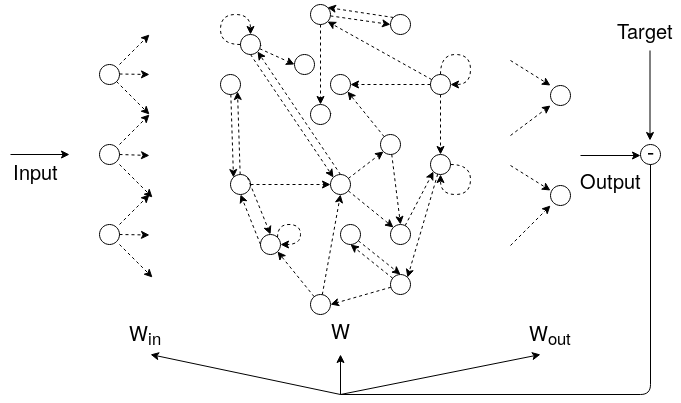
\includegraphics[width=0.7\linewidth]{immagini/RNN(1).png}
	\caption{Metodo di allenamento basato  su discesa di gradiente che adatta tutti i pesi delle connessioni.}
	\label{fig:RNN}
\end{figure} 

Le reti neurali ricorrenti si presentano come strumenti molto promettenti per processare sequenze temporali non lineari per due ragioni. Innanzitutto rappresentano una approssimazione dei sistemi dinamici, in secondo luogo si avvicinano al modello del cervello biologico grazie alle connessioni ricorrenti.\\
Tuttavia vi sono delle problematiche legate all'apprendimento evidenziate in \cite{RCapproch:paper} e riportate qui di seguito:
\begin{itemize}
	\item Non può essere garantita la convergenza del metodo di allenamento a discesa di gradiente, vi sono dei punti in cui le informazioni sul gradiente possono essere mal definite.
	\item L'aggiornamento di un solo parametro può essere computazionalmente costoso,
	cioè possono essere necessari molti cicli di aggiornamento. Questo comporta lunghi tempi di addestramento che rendono le RNN modelli convenienti utilizzando solo poche unità.
	\item È molto difficile apprendere relazioni che richiedono molta memoria perché le informazioni fornite dal gradiente subiscono una dissolvenza esponenziale nel tempo.
	\item  Gli algoritmi di apprendimento necessitano di  profonde conoscenze ed esperienza per essere applicati con successo.
\end{itemize}
In questa situazione di lento progresso, nel 2001 un nuovo approccio al design e all'allenamento delle RNN, noto come Reservoir Computing, venne proposto indipendentemente da Wolfgang Maass \cite{w} e da Herbert Jaeger \cite{h}.







\chapter{Echo State Network}\label{cap:modello}

\section{Il modello di base}
Come evidenziato nella sezione \ref{sec:rnn} le diverse problematiche relative all'allenamento delle reti neurali ricorrenti hanno portato allo sviluppo del \textit{Reservoir Computing }. L'approccio del \textit{Reservoir Computing} differisce dalla tecnica di apprendimento citata in precedenza perché crea una separazione concettuale e computazionale tra una parte dinamica chiamata  \textit{reservoir} ed una parte chiamata \textit{readout}. Il \textit{reservoir} è una  rete neurale ricorrente che opera come funzione di espansione non lineare, mentre il \textit{readout} produce l'output desiderato dall'espansione. \\

Una \textit{Echo State Network} consiste in un livello di input di $N_u$ unità, un insieme di $N_r$ unità nascoste che compongono il suddetto \textit{reservoir} e un livello di output di $N_y$ unità tipicamente lineari e non ricorrenti che formano il \textit{readout}.
Le equazioni che descrivono la computazione sviluppata da una ESN sono:
\begin{equation}\label{attivazioneesn}
\mathbf{x}(\mathit{t})= \mathit{f}_\mathit{x} (\mathbf{u}(\mathit{t}), \mathbf{x}(\mathit{t} - 1)) = f(\mathbf{W_{in}}u(\mathit{t}) + \mathbf{Wx}(\mathit{t - 1} ) + \mathbf{b} )
\end{equation}
\begin{equation}\label{output}
\mathbf{y}(\mathit{t})=\mathit{f_{y}}(\mathbf{x}(\mathit{t}) )= \mathbf{W_{out}}\mathbf{x}(\mathit{t})
\end{equation}
La separazione concettuale che caratterizza le \textit{echo state network} è basata sulla comprensione dei diversi scopi che assumono $\mathit{f_{x}}$ e $\mathit{f_{y}}$:
\begin{itemize}
	\item $\mathit{f_{x}}$ espande la storia dell'input $\mathbf{u}\mathit{(t)}, \mathbf{u}\mathit{(t-1)}$,... in uno spazio degli stati del \textit{reservoir}  $\mathbf{x}\mathit{(t)} \in \mathds{R}^{N_x}$,
	\item mentre $\mathit{f_{y}}$ combina i segnali ricevuti dai neuroni $\mathbf{x}(\mathit{t})$ per ottenere gli output attesi $\hat{\mathbf{y}}(\mathit{t})$ .\\
\end{itemize}
  
La principale caratteristica del RC e quindi delle ESN è che la parte ricorrente della rete può non essere allenata dopo essere inizializzata secondo alcune proprietà facili da soddisfare. L'allenamento si riduce dunque alla sola parte non ricorrente, si riducono così i costi computazionali che gravavano sul design delle RNN. Di seguito in figura \ref{fig:RC} viene illustrato il design e l'allenamento di una ESN.\\

\begin{figure}[h!]
	\centering 
	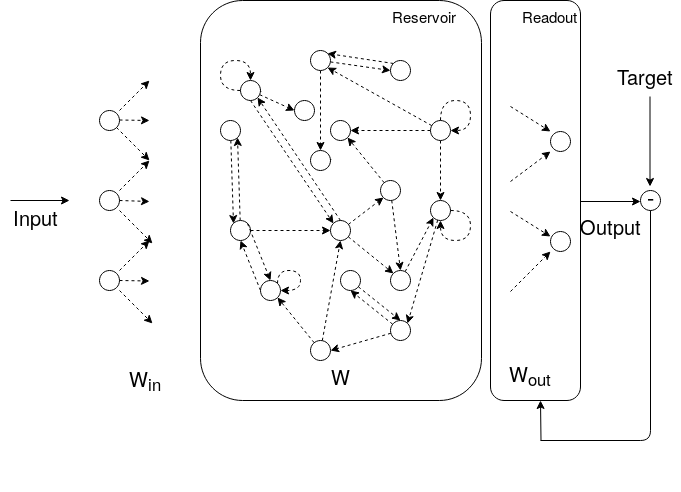
\includegraphics[width=0.7\linewidth]{immagini/RC.png}
	\caption{\textit{Reservoir Computing} e allenamento del readout.}
	\label{fig:RC}
\end{figure}

Ciò significa che $\mathbf{\mathbf{W_{in}}}$ e $\mathbf{\mathbf{W}}$ sono fisse e $\mathbf{\mathbf{W_{out}}}$ varia in base all'allenamento. Tuttavia non tutte le scelte di $\mathbf{\mathbf{W_{in}}}$ e $\mathbf{\mathbf{W}}$ producono una ESN valida, il \textit{reservoir} deve essere un eco ("echo") della storia dell'input, cioè le dinamiche del \textit{reservoir} devono dipendere asintoticamente solo dai segnali di input.


\section{Le funzioni di attivazione}
Le funzioni di attivazioni alle quali si fa riferimento nella formula \ref{attivazioneesn} possono essere diverse, tra queste:
\begin{itemize}
	\item la funzione identità : $f_{id}(x)=x$ (\ref{att:(a)})
	\item la funzione logistica : $f_{logistic}(x)=  {1 \over 1+ e^{-x} }$ (\ref{att:(b)})
	\item la tangente iperbolica : $f_{tanh}(x)=  {e^{x}- e^{-x} \over e^{x}+ e^{-x} }$ (\ref{att:(c)})
\end{itemize}

\begin{figure}[h!]
	\centering
	\begin{subfigure}[b]{0.30\textwidth}
		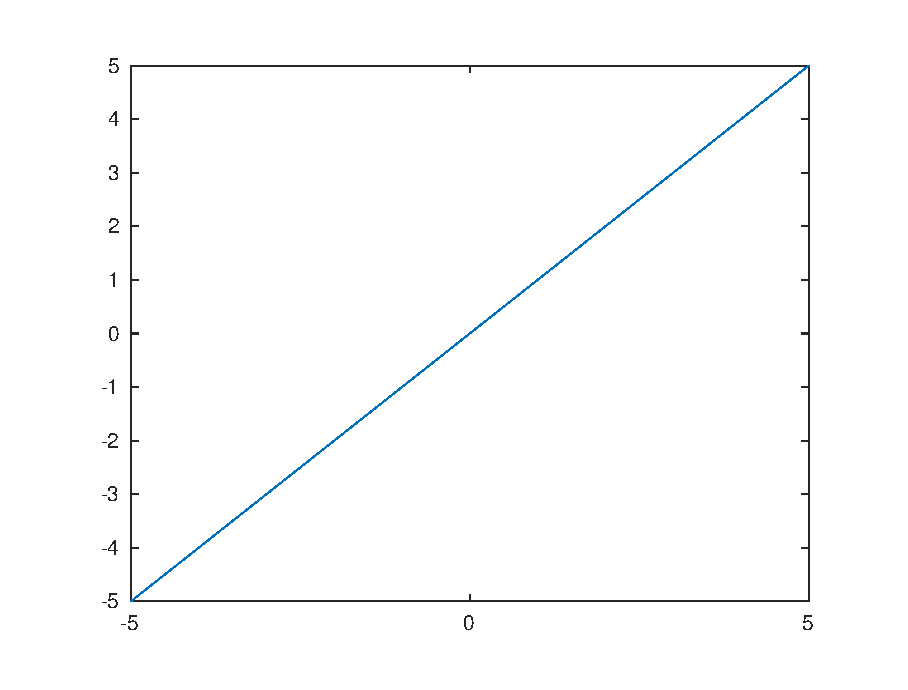
\includegraphics[width=\linewidth]{immagini/id}
		\caption{Funzione identità}
		\label{att:(a)}
	\end{subfigure}%
	\begin{subfigure}[b]{0.30\textwidth}
		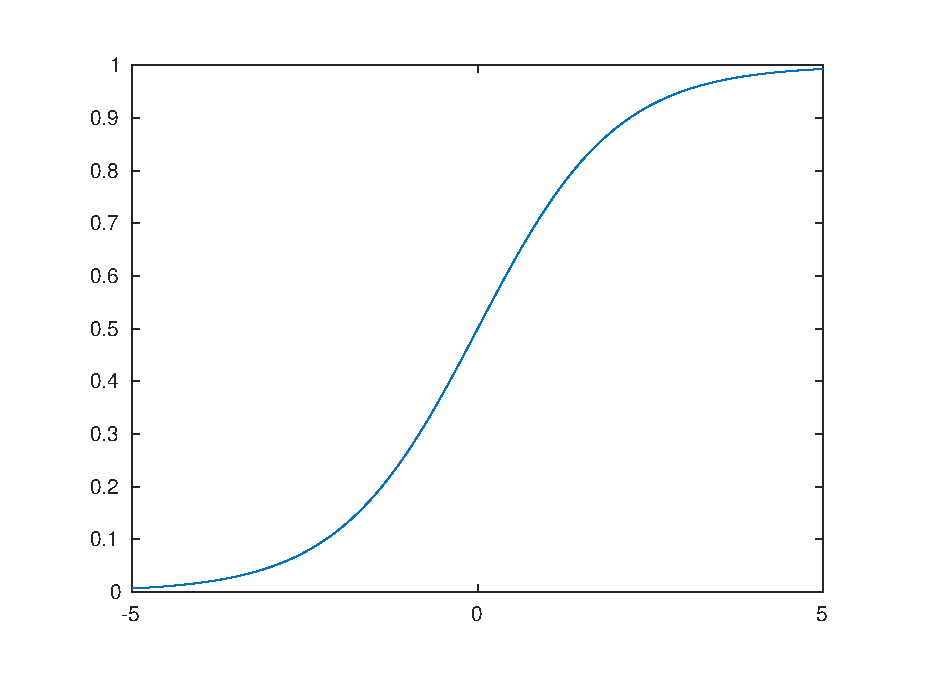
\includegraphics[width=\linewidth]{immagini/logistic}
		\caption{Funzione logistica}
		\label{att:(b)}
	\end{subfigure}%
	\begin{subfigure}[b]{0.30\textwidth}
		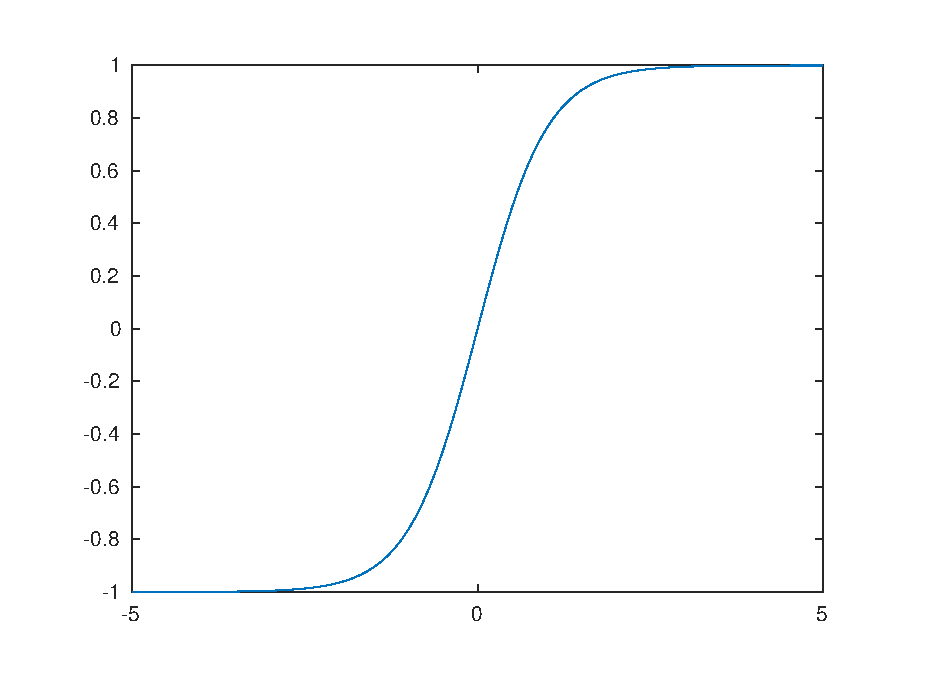
\includegraphics[width=\linewidth]{immagini/tanh}
		\caption{Tangente iperbolica}
		\label{att:(c)}
	\end{subfigure}%
	\caption{Funzioni di attivazione comuni.}\label{fattivazioni}
\end{figure}

La funzione logistica e la tangente iperbolica sono le più usate, l'idea è che si può mappare ogni numero reale in un numero nell'intervallo $[0,1]$ e rispettivamente in $[-1,1]$, in questo modo si può dimostrare che una combinazione di queste funzioni può approssimare ogni funzione non lineare.\\

\section{Leaking integration}
Le unità nelle reti  sigmoidali standard non hanno memoria; il loro valore ad un tempo $n+1$ dipende solo parzialmente ed indirettamente dai valori precedenti. Perciò queste reti si adattano al meglio per sistemi discreti nel tempo, d'altra parte è difficile l'apprendimento di dinamiche lente come onde sinusoidali molto lente. Per apprendere sistemi lenti e variabili in uno spazio continuo è più adeguato utilizzare delle reti con dinamiche continue. Per questo già in 
\cite{h} viene introdotto un approccio ibrido che usa reti discrete nel tempo che approssimano delle reti continue grazie alle unità con \textit{leaky integration}.
In questo caso una semplificazione dell'equazione per il calcolo dello stato delle unità è la seguente:

\begin{equation} \label{attivazionelr}
\mathbf{x}(\mathit{t})=(1-\alpha) \mathbf{x}(\mathit{t - 1} ) + \alpha \mathit{f}_\mathit{x} (\mathbf{u}(\mathit{t}), \mathbf{x}(\mathit{t} - 1)) = 
\end{equation}
\begin{displaymath}
(1-\alpha) \mathbf{x}(\mathit{t - 1} ) + \alpha f(\mathbf{W_{in}}u(\mathit{t}) + \mathbf{Wx}(\mathit{t - 1} ) + \mathbf{b} )
\end{displaymath}  

dove $\alpha \in (0,1]$ è il \textit{leaking decay rate}, se si  
imposta $\alpha=1$ si ottiene una ESN standard.

\section{Echo State Property}
Una ESN valida soddisfa la cosiddetta \textit{Echo State Property} (ESP) (Jager,2001). Questa dice che lo stato in cui la rete si trova dopo l'analisi di una lunga sequenza di input dipende solo dalla sequenza stessa. La dipendenza dallo stato iniziale della rete è progressivamente persa quando la lunghezza della sequenza di input tende all'infinito. Analogamente, lo stato corrente della rete $\mathbf{x}(\mathit{t})$ è una funzione della storia dell'input indipendentemente dai valori iniziali dello stato. In formule la ESP può essere espressa come segue:
\begin{displaymath}
\forall s_n(\mathbf{u}) = [\mathbf{u}(1),...,\mathbf{u}(\mathit{n})] \in (\mathbb{R}^{N_u})^n sequenza\ di\ input\ di\ lunghezza\ n,
\end{displaymath}
\begin{equation}\label{ESP}
\forall \mathbf{x}, \mathbf{x'} \in \mathbb{R}^{N_r}:
\end{equation}
\begin{displaymath}
 \Vert \mathit{f_x}(s_n(\mathbf{u}), \mathbf{x}) - \mathit{f_x}(s_n(\mathbf{u}), \mathbf{x'}) \Vert \rightarrow 0\ per\ \mathit{n} \rightarrow \infty
\end{displaymath}
che significa che la differenza tra gli stati che la rete assume dopo che viene valutata una sequenza di input di lunghezza $n$ tende a zero al tendere di $n$ ad infinito, per ogni scelta iniziale dello stato.\\
Jaeger ha fornito due condizioni, rispettivamente necessaria e sufficiente, affinchè una ESN goda di questa proprietà. La condizione necessaria è che il raggio spettrale, ovvero il maggiore degli autovalori in modulo, della matrice dei pesi del \textit{reservoir} sia minore di uno.
\begin{equation}\label{raggiospettrale}
\rho(\mathbf{W})<1
\end{equation}
Se questa condizione viene violata, il \textit{reservoir} è localmente asintoticamente instabile nello stato $\mathbf{0} \in \mathbb{R}^{N_r}$ e la \textit{echo state property} non può essere garantita se la sequenza nulla è un input ammissibile per il sistema.\\
La condizione sufficiente per la validità della proprietà è che il massimo valore singolare di \textbf{W} sia minore di uno:
\begin{equation}\label{raggiospettrale2}
\sigma(\mathbf{W}) <1
\end{equation}
Ciò assicura la stabilità globale del sistema e la presenza di "stati echo", garantendo così la \textit{echo state property}.\\
Una caratteristica molto importante evidenziata in \cite{Markovianfactor:paper}  è la contrattività delle dinamiche dello stato.\\
La contratività della funzione di transizione dello stato $\mathit{f_x}$ è una condizione sufficiente ma non necessaria per garantire la ESP.


\chapter{Implementazione}\label{cap:implementazione}
Seguendo gli studi sviluppati in \cite{praticalguide}, vengono presentate le scelte progettuali fatte per l'implementazione e l'uso del \textit{reservoir} e del \textit{readout}.
\section{Inizializzazione del Reservoir}
Dato il modello delle RNN, il \textit{reservoir} è definito dalla tupla $(\mathbf{W_{in}},\mathbf{W}, \alpha)$. Le matrici dei pesi delle connessioni e dei pesi di input sono generate in modo random secondo dei parametri di cui si discute in seguito, e il \textit{leaking rate} $\alpha$ è selezionato come parametro libero.\\
Analogamente a quanto viene fatto nella letteratura, quelli che per semplicità vengono chiamati parametri globali in questa sezione potrebbero essere chiamati iper-parametri, poiché non rappresentano direttamente i pesi delle connessioni ma regolano la loro distribuzione.\\
I parametri globali del \textit{reservoir} sono: la dimensione $N_r$,la sparsità, ovvero la distribuzione degli elementi non nulli, e il raggio spettrale di $\mathbf{W}$; lo \textit{scaling} di $\mathbf{W_{in}}$ ; ed il \textit{leaking rate} $\alpha$.
I dettagli di ciascuno di queste scelte di design vengono illustrate in seguito.
Per inizializzare un \textit{reservoir} si  invoca la funzione \textit{weightMatrix()} con gli opportuni parametri.\\
\\
\lstinputlisting[frame=single]{code/weightMatrix.m}

\subsection{Dimensione del Reservoir}
Un parametro fondamentale per il modello \ref{attivazioneesn} è $N_r$, il numero delle unità del \textit{reservoir}. In genere più è grande il \textit{reservoir}, migliore è la performance ottenuta, tenendo conto delle tecniche di regolarizzazione appropriate per evitare l'\textit{overfitting}. Poiché allenare ed applicare le ESN è computazionalmente economico rispetto alle altre reti neurali ricorrenti, non è insolito trovare dei reservoir di dimensioni dell'ordine di $10^4$.\\
Più è grande lo spazio dei segnali del \textit{reservoir} $\mathbf{x}(n)$, più facile è trovare una combinazione lineare dei segnali per approssimare $\mathbf{y}_{target}(n)$. Il \textit{reservoir} può essere troppo grande quando il \textit{task} è banale oppure quando non si hanno molti dati disponibili, ad esempio $T< 1+ N_u +N_r$.\\
Generalmente nell'ambito accademico la dimensione del \textit{reservoir} viene limitata per convenienza e per compatibilità di risultati; inoltre buoni parametri sono trasferibili a \textit{reservoir} di dimensioni maggiori,quindi può essere conveniente selezionare i parametri globali con \textit{reservoir} ridotti e poi trasferirli a quelli più grandi.\\
Un limite inferiore per la dimensione del \textit{reservoir} può essere considerato il numero di valori reali che il reservoir deve ricordare dall'input per realizzare con successo il \textit{task}. Il massimo numero di valori conservati in una ESN non può essere superiore di $N_r$.
il parametro che indica la dimensione del \textit{reservoir}  passato alla funzione \textit{weightMatrix()} è $nr$.

\subsection{Sparsità del Reservoir}
Nelle prime pubblicazioni riguardanti le ESN si raccomanda di realizzare \textit{reservoir} con connessioni sparse, cioè con le matrici $\mathbf{W_{in}}$ e $\mathbf{W}$ aventi la maggior parte degli elementi uguali a zero.
In generale questo parametro non influenza la performance così tanto ed ha una bassa priorità nell'ottimizzazione, come viene dimostrato anche in \cite{Markovianfactor:paper}.\\
La sparsità fa si che l'aggiornamento della matrice sia più rapido, velocizzando quindi la computazione. Matrici densamente connesse potrebbero rallentare la computazione, soprattutto in base al numero di unità di attivazione considerate, quando la dimensione del \textit{reservoir} è grande si può decidere di generare $\mathbf{W_{in}}$ e $\mathbf{W}$ secondo la stesso tipo di distribuzione ma una rispettivamente densa e sparsa. In particolare nell'implementazione fornita si può scegliere la distribuzione tra quella uniforme e quella normale associando, rispettivamente, le stringhe '\textit{ud}' e '\textit{nd}' al parametro \textit{dist}. Inoltre si può esprimere la densità delle connessioni del \textit{reservoir} attraverso il parametro $\mathit{density\_con}$,il cui valore va da $0$ a $1$, dove con $1$ si indica una matrice completamente connessa. 

\subsection{Raggio spettrale}
Uno dei principali parametri delle ESN è il raggio spettrale della matrice dei pesi delle connessioni, cioè il massimo tra i valori assoluti degli autovalori della matrice. Questo parametro scala la matrice $\mathbf{W}$, o visto alternativamente scala l'ampiezza della distribuzione dei parametri diversi da zero.\\
Viene generata in modo random la matrice \textbf{W}, viene calcolato il suo raggio spettrale $\rho(\mathbf{W})$, infine \textbf{W} viene divisa per $\rho(\mathbf{W})$ così da ottenere una matrice con raggio spettrale unitario da poter moltiplicare per il raggio spettrale desiderato. Si ricorda che questo ultimo deve essere minore di uno affinché valga la \textit{Echo State Property}.\\
Come principio guida, $\rho(\mathbf{W})$ dovrebbe essere scelto grande per i \textit{task} per i quali è richiesto una storia dell'input vasta , piccolo per i \textit{task} il cui output corrente dipende dalla storia recente.
Il valore del raggio spettrale desiderato è espresso dal parametro \textit{rho}.

\subsection{Input scaling}
Lo \textit{scaling} dei pesi della matrice di input è un altro valore chiave da ottimizzare in una Echo State Network. Per $\mathbf{W_{in}}$ generate con distribuzione uniforme generalmente ci si riferisce all'\textit{input scaling a} come al modulo degli estremi dell'intervallo $[-a;a]$ dal quale vengono selezionati i valori di $\mathbf{W_{in}}$; per le matrici generate con distribuzione normale si prende la deviazione standard come misura di \textit{scaling}.\\
In questa implementazione, per avere un numero esiguo di parametri liberi, tutte le colonne di $\mathbf{W_{in}}$ vengono scalate insieme in base ad un unico valore. In alternativa si può ottimizzare separatamente il valore di \textit{input \textit{scaling}} relativo alla colonna del \textit{bias}, oppure si possono scalare le colonne di $\mathbf{W_{in}}$ separatamente in base a come queste contribuiscono al \textit{task}. A seconda delle impostazioni il numero di parametri liberi per $\mathbf{W_{in}}$  varia da 1 a $N_u + 1$.\\
Nelle prime pubblicazioni venne suggerito di scalare e traslare i dati di input, ottimizzando queste operazioni. Lo stesso effetto può essere raggiunto scalando i pesi di input e il \textit{bias}, rispettivamente. Queste operazioni sono molto utili poiché permettono di avere dei valori limitati per i dati di input. \\
Per \textit{task} molto lineari $\mathbf{W_{in}}$ dovrebbe essere piccolo, permettendo alle unità di operare intorno allo zero dove la funzione di attivazione $tanh$, funzione di attivazione scelta in questa implementazione, è quasi lineare. Par  $\mathbf{W_{in}}$ con valori grandi , le unità si saturano facilmente vicino al loro valore $-1$ o $1$, agendo in modo non lineare. È chiaro che l'\textit{input scaling}, insieme al valore $\rho(\mathbf{W})$, determina quanto lo stato corrente $\mathbf{x}(t)$ dipende dall'input corrente $\mathbf{u}(t)$ e quanto dallo stato precedente  $\mathbf{x}(t-1)$. Nell'implementazione il valore dell'\textit{input scaling} viene indicato da $\mathit{scale\_in}$.

\subsection{Leaking Rate}
La variabile \textit{alpha} esprime il valore del \textit{leaking rate} come visto in \ref{attivazionelr} ed indica la velocità con cui vengono aggiornate le dinamiche del \textit{reservoir}. Sebbene questo parametro viene maggiormente utilizzato nel calcolo dello stato del \textit{reservoir} viene presentato qui  poiché si deve tener conto di questo valore nel momento in cui viene riscalata la matrice dei pesi $\mathbf{W}$ come dimostrato in \cite{leakingintegrator}. 



\section{Calcolo dello stato del Reservoir}
Per calcolare lo stato del reservoir è necessario invocare la funzione, riportata sotto, \textit{setReservoir()}. Questa prende come parametri le informazioni relative al \textit{task} e le matrici che rappresentano il \textit{reservoir}, inizializzate come espresso sopra.
Può prendere in ingresso dei parametri opzionali che rappresentano rispettivamente il valore del \textit{leaking rate} e dell'\textit{input bias}. Viene applicata la \ref{attivazionelr} per il calcolo dello stato del \textit{reservoir} e viene eliminato il numero di stati \textit{transient}  come espresso nella definizione del \textit{task}.\\
Ciò significa che i valori iniziali $\mathbf{x}(n)$ non vengono considerati per l'allenamento del \textit{readout} e vengono scartati in quanto influenzati dallo stato iniziale $\mathbf{x}(0)$, che tipicamente è $\mathbf{x}(0)=0$. Questo introduce uno stato iniziale non naturale difficile da raggiungere quando la rete comincia ad adattarsi al \textit{task}. Il numero di \textit{step} da saltare dipende dalla memoria della rete e tipicamente è dell'ordine di decine di centinaia. Tuttavia se il \textit{task} è composto da molte sequenze corte il \textit{transient} iniziale è la normale modalità di lavoro della ESN ed in questi casi eliminare gli stati iniziali può essere pericoloso.\\
Invece questo aspetto diventa fondamentale se si vogliono rendere indipendenti le sequenze, ad esempio quelle associate a \textit diversi.
\lstinputlisting[frame=single]{code/setReservoir.m}


\section{Allenamento del Readout}
Per questa implementazione si prende in considerazione un \textit{readout} lineare, senza connessioni di \textit{feedback}.\\
Un \textit{readout} lineare può essere descritto con la seguente equazione
\begin{equation} \label{eq:readout}
\mathbf{Y}= \mathbf{W_{out}X}
\end{equation}
dove:
\begin{itemize}
	\item $\mathbf{Y} \in \mathbb{R}^{N_y*T}$ sono tutti gli $\mathbf{y}(n)$;
	\item $\mathbf{X} \in \mathbb{R}^{(1+N_r)*T}$ sono tutti gli $[\mathbf{x}(n);1]$
	\item $\mathbf{W_{out}}$ sono i pesi ottimi che minimizzano l'errore tra $\mathbf{y}(n)$ e $\mathbf{y_{target}}(n)$
\end{itemize}
Nel caso in cui si volessero connettere i pesi di input al \textit{readout} si avrebbe la matrice $\mathbf{X} \in \mathbb{R}^{(1+N_u+N_r)*T}$, formata da tutti i $[\mathbf{x}(n);\mathbf{u}(n);1]$.\\
Trovare i pesi ottimi $\mathbf{W_{out}}$ che minimizzino l'errore tra $\mathbf{y}(n)$ e $\mathbf{y_{target}}(n)$ consiste nel risolvere un sistema di equazioni lineari del tipo:
\begin{equation} \label{eq:readout_targ}
\mathbf{Y_{target}}= \mathbf{W_{out}X}
\end{equation}
Per allenare il \textit{readout} si deve invocare la funzione $\mathit{train\_readout()}$, nelle sottosezioni successive vengono illustrati due approcci diversi per la risoluzione del sistema.

\subsection{Regolarizzazione di Tikhonov}
La più diffusa e stabile soluzione per \ref{eq:readout_targ} in questo contesto è la regolarizzazione di \textit{Tikhonov} o \textit{Ridge Regression}, in formula:
\begin{equation} \label{eq:tikhonov}
\mathbf{W_{out}}= \mathbf{Y_{target}X^T} (\mathbf{XX^T} + \beta\mathbf{I})^{-1}
\end{equation}
dove $\beta$ è il coefficiente di regolarizzazione.\\
Per misurare la qualità della soluzione prodotta dall'allenamento è consigliabile controllare i pesi ottenuti di $\mathbf{W_{out}}$, grandi pesi indicano che $\mathbf{W_{out}}$ amplifica piccole differenze tra le dimensioni di $\mathbf{x}(t)$ e può essere molto sensibile nelle situazioni diverse dalle esatte condizioni nelle quali la rete è stata allenata. Questo problema si accentua nel caso in cui la rete riceve il suo output come successivo input.\\
Per contrastare questi effetti viene introdotta la parte di regolarizzazione  $\beta\mathbf{I}$. Per illustrare l'equazione risolta con la \textit{ridge regression} viene considerato il RMSE (\textit{root mean squared error}) come misura di errore:
\begin{equation} \label{eq:tikhonov2}
\mathbf{W_{out}}= \underset{\mathbf{W_{out}}}{\arg\min} \frac{1}{N_y} \sum\limits_{i=1}^{N_y} \biggl( \sum\limits_{n=1}^{T} (y_i(n)-y_{i_{target}}(n))^2 + \beta \| w_{i_{out}} \|^2 \biggr)
\end{equation}
con $w_{i_{out}}$ che indica la \textit{i-esima} riga di $\mathbf{W_{out}}$ e $\|\cdot\|$ la norma euclidea. È evidente il compromesso che si ha tra avere un basso \textit{training error} e pesi di output piccoli, ed è regolato proprio dal parametro di regolarizzazione $\beta$.
Il coefficiente di regolarizzazione ottimo $\beta$ dipende dall'istanza di $\mathbf{W}$, quindi è buona norma scegliere questo parametro attraverso la validazione.\\
Settare $\beta$ uguale a \textit{zero} rimuove la regolarizzazione: la funzione in \ref{eq:tikhonov2} diventa uguale al semplice calcolo del RMSE(\textit{root mean squared error}),
rendendo la regolarizzazione di \textit{Tikhononov} una generalizzazione della regressione lineare.\\
La soluzione con $\beta=0 $ diventa:
\begin{equation} \label{eq:linearregression}
\mathbf{W_{out}}= \mathbf{Y_{target}X^T} (\mathbf{XX^T})^{-1}
\end{equation}
Nella pratica, tuttavia, fissare $\beta=0 $ spesso causa instabilità numerica quando si inverte $(\mathbf{XX^T})$ in \ref{eq:linearregression}, è per questo che si raccomanda di usare per la selezione di $\beta$ una scala logaritmica che non raggiunge lo \textit{zero} o di usare la pseudoinversa invece che l'inversa come mostrato di seguito.

\subsection{Soluzione con pseudoinversa}
Una soluzione semplice per la risoluzione del sistema visto prima è:
\begin{equation} \label{eq:pseudoinversa}
\mathbf{W_{out}}= \mathbf{Y_{target}X^+}
\end{equation}
dove $\mathbf{X^+}$ è la pseudoinversa di \textit{Moore-Penrose} di $\mathbf{X}$. Se $\mathbf{XX^T}$ è invertibile questa formula diventa uguale alla \ref{eq:linearregression}, ma funziona anche quando non lo è.\\
Tuttavia, ha un elevato costo in memoria per grandi matrici $\mathbf{X}$, dunque si deve limitare la dimensione del \textit{reservoir} e/o il numero di esempi di \textit{training} $T$.
Poichè non si ha la regolarizzazione il sistema di equazioni lineari \ref{eq:readout_targ} deve essere sovraddeterminato, cioè $ 1+N_u+ N_r << T$. In altre parole, il \textit{task} deve essere difficile in relazione alla capacità del \textit{reservoir} così che non avvenga l'\textit{overfitting}.\\
In molte librerie viene fornita una implementazione della pseudoinversa, tuttavia ogni implementazione varia nella precisione, nell'efficienza computazionale e nella stabilità numerica. Per \textit{task} di alta precisione, si deve controllare se la regressione $\mathbf{(Y_{target} -W_{out}X)X^+}$ sull'errore $\mathbf{Y_{target} -W_{out}X}$ è effettivamente uguale a \textit{zero}, e aggiungerla a $\mathbf{W_{out}}$ nel caso non lo sia. Questo trucco computazionale non dovrebbe funzionare in teoria ma a volte funziona in partica in Matlab, probabilmente a causa di qualche ottimizzazione interna.



\chapter{Test}\label{cap:test}
In questo capitolo viene testata la rete neurale implementata attraverso il \textit{task} NARMA e vengono confrontati i risultati ottenuti con quelli della letteratura.

\section{$\mathbf{10^{th}}$ order NARMA system}
Questo \textit{task} consiste nella predizione di un sistema di $10^{th}$ ordine di media mobile autoregressivo non lineare. Il \textit{task} è stato introdotto in Atiya e Palos (2000) ed è stato trattato con le ESN in Jaeger (2002) e in Cernansk\'y e Ti\v{n}o (2008). L'input del sistema è una sequenza di elementi $\mathbf{u}(n)$ scelti secondo una distribuzione uniforme in $[0,0.5]$. L'output del sistema è calcolato come:

\begin{equation}\label{narma}
	\bar{\mathbf{y}}(n) = 0.3\bar{\mathbf{y}}(n-1) + 0.05\bar{\mathbf{y}}(n-1)\biggl( \sum_{i=1}^{10}\bar{\mathbf{y}}(n - i)\biggr) + 1.5 \mathbf{u}(n-10)\mathbf{u}(n-1) +0.1 .
\end{equation}

Dato il valore di input $\mathbf{u}(n)$, il \textit{task} è di predire il corrispondente valore di $\bar{\mathbf{y}}(n)$. Il \textit{training set} è formato da $N_{train}=2200$ esempi \textit{input-target},dei quali $N_{transient}=200$ sono di \textit{transient} iniziale. Una sequenza di lunghezza $N_{test}=2000$ viene usata per il test.\\
Il \textit{task} viene generato attraverso la funzione \textit{genetateTask()}, passando come argomento \textit{Tasks.narma}, questa funzione permette di generare tutti i \textit{task} che sono elencati nell'enumerazione \textit{Tasks}, questi ultimi vengono creati secondo dei criteri ben precisi in modo da poter fornire alla rete tutte le informazioni necessarie. Per verificare che un \textit{task} abbia tutti i campi necessari per essere ben definito è utilizzata la funzione \textit{isTask()}.

\section{ESNtrain() ed ESNtest()}
Per facilitare l'uso della rete sviluppata viene fornita una funzione chiamata \textit{ESNtrain()}. La funzione si occupa dell'inizializzazione delle matrici dei pesi, del calcolo dello stato del \textit{reservoir} e del \textit{training} del \textit{readout} invocando le funzioni illustrate nel capitolo \ref{cap:test}. A questa funzione devono essere passati come argomenti un \textit{task} valido e tutti i parametri che si intendono usare nella rete, qualora questi non fossero presenti vengono utilizzati dei parametri standard illustrati nella tabella sottostante.
\begin{table}[h]
	\begin{center}
	 \begin{tabular}{|l|c|r|}
	 	\hline
	 	\textbf{parametri}		&\textbf{nome parametro}&   \textbf{valore default}\\
	 	\hline
	 	input scaling			&  \textit{scale\_in}	&   0.1\\
	 	\hline
	 	unità reservoir 		&  \textit{nr}          &   100\\
	 	\hline
	 	tipo di distribuzione	&  \textit{dist}        &   'ud'\\
	 	\hline
	 	densità connessione		&  \textit{density\_con}&   1\\
	 	\hline
	 	raggio spettrale		&  \textit{rho}			&   0.9\\
	 	\hline
	 	leaky integrator		&  \textit{alpha}		&   1\\
	 	\hline
	 	input bias				&  \textit{bias}		&   1\\
	 	\hline
	 	par regolazizzazione	&  \textit{lambda}		&   0\\
	 	\hline
	 	misura errore			&  \textit{error}		&   'mse'\\
	 	\hline
	 	risultati test			&  \textit{test}		&   true\\
	 	\hline
	 \end{tabular}
	\end{center}
	\caption{Parametri default \textit{ESNtrain()}}
\end{table}

In particolare si ha il parametro \textit{test} che se settato a \textit{true} permette di ottenere anche il risultato di test,eseguito dopo il \textit{training}. Se viene usata questa opzione bisogna far attenzione a non usare il valore di test per la scelta del modello, in questo caso infatti la \textit{model selection} verrebbe compromessa. Per il test della rete deve essere usata la funzione \textit{ESNtest()}. Questa funzione prende in ingresso il \textit{task} ed eventualmente altri parametri per la realizzazione della rete, infatti si può decidere se passare o meno come parametri un \textit{reservoir} ed un \textit{readout} allenato. Nel primo caso viene eseguita solo una fase di test, altrimenti viene inizializzata un'altra rete secondo i parametri passati come argomento; quest'ultima operazione assume un certo valore soprattutto nel caso in cui i parametri passati come argomento sono quelli di una \textit{model selection} precedente.

\section{Risultati}
Per poter ottenere dei risultati confrontabili con quelli in \cite{Markovianfactor:paper} viene fatta una \textit{model selection} al variare del parametro \textit{rho}, ovvero del raggio spettrale. Nelle figure successive sono mostati in ordine i valori dell'errore di train, dell'errore di test ottenuto con la funzione \textit{ESNtrain()}, di quello di test ottenuto con la funzione \textit{EStest()} avente come parametri rispettivamente quelli ottenuti della \textit{model selection} ed il \textit{reservoir} ed il \textit{readout} prodotti in precedenza.

\begin{figure}[h!]
	\centering 
	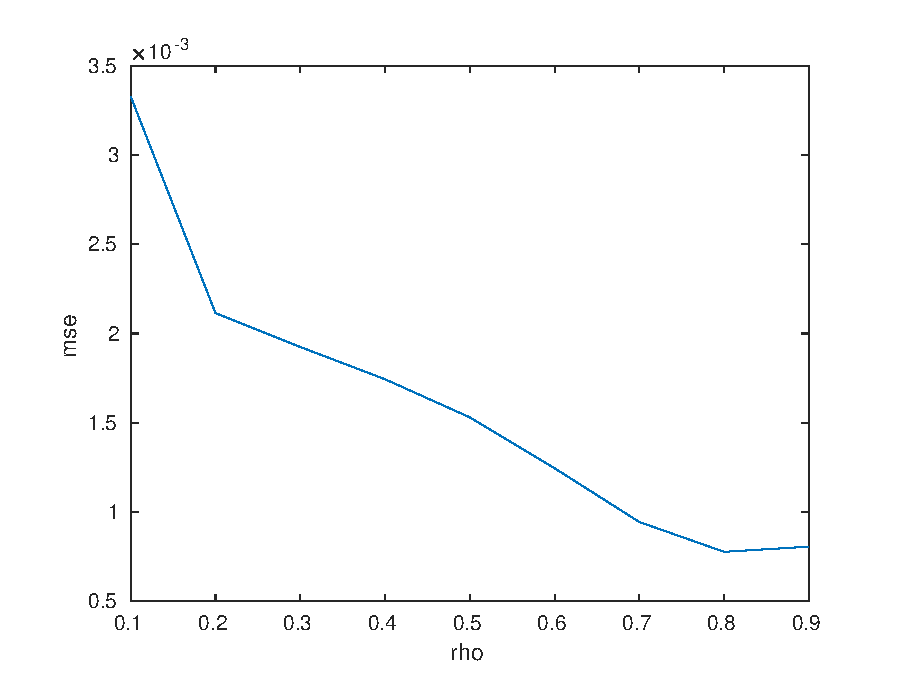
\includegraphics[width=0.7\linewidth]{immagini/trainingerror.eps}
	\caption{Training error generato da \textit{ESNtrain().}}
	\label{fig:trainingerror}
\end{figure}
L'errore di training è naturalmente più basso dell'errore di test che riflette comunque lo stesso andamento.\\
\begin{figure}[H]
	\centering 
	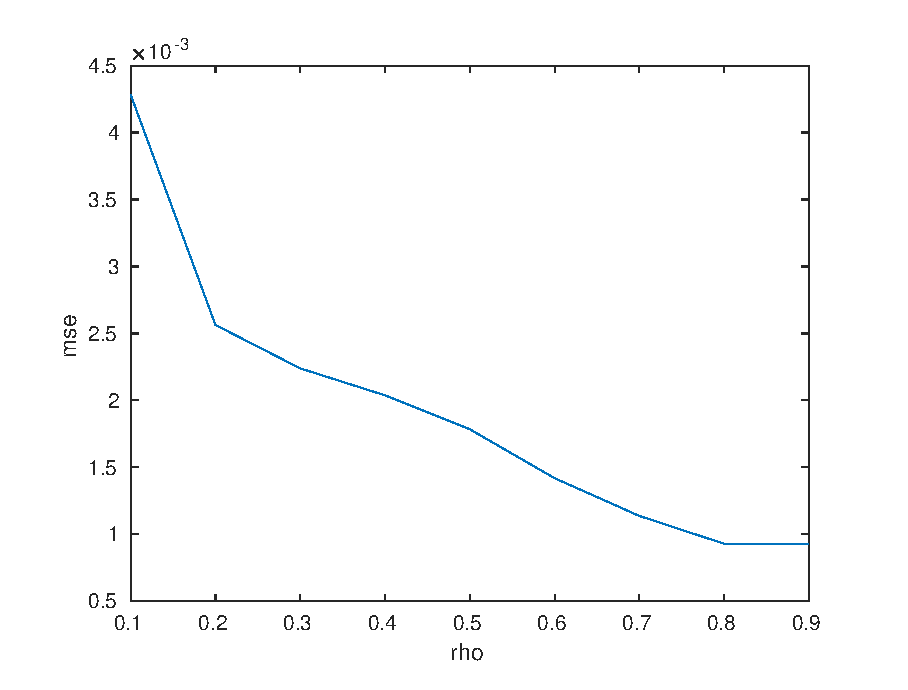
\includegraphics[width=0.6\linewidth]{immagini/testaftertrain}
	\caption{Test error generato da \textit{ESNtrain()} dopo l'allenameto del readout.}
	\label{fig:testaftertrain}
\end{figure}
\begin{figure}[H]
	\centering 
	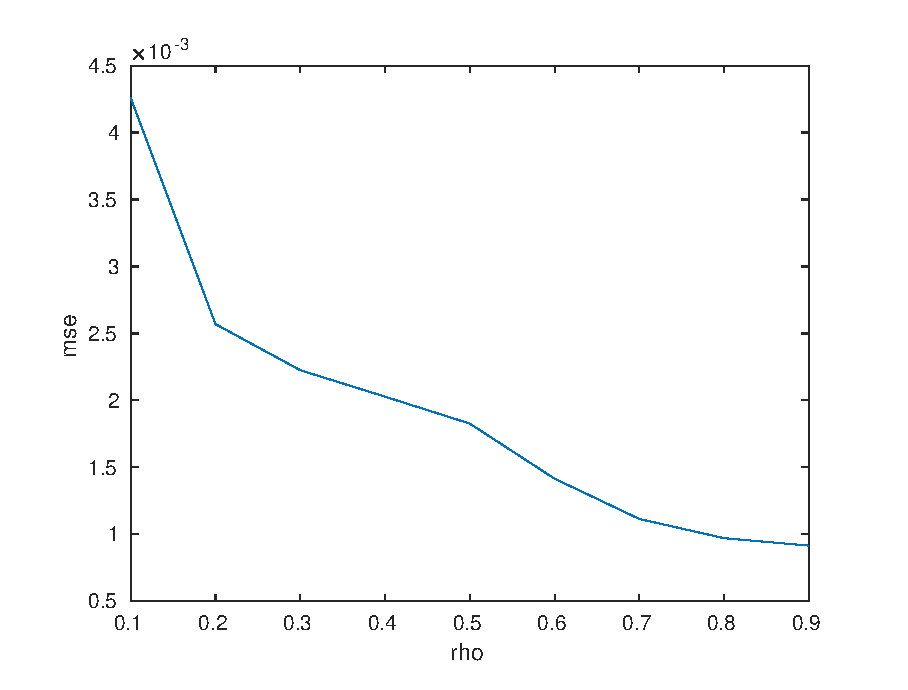
\includegraphics[width=0.6\linewidth]{immagini/testnewtrain}
	\caption{Test error generato da \textit{ESNtest()} dopo una nuova inizializzazione di \textit{reservoir}.}
	\label{fig:testnewtrain}
\end{figure}
\begin{figure}[H]
	\centering 
	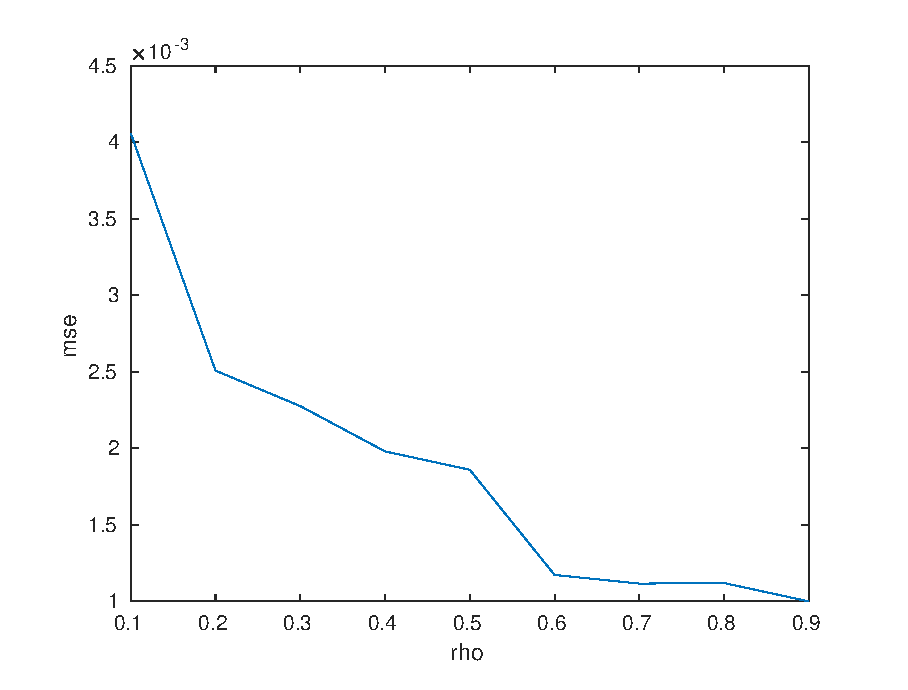
\includegraphics[width=0.6\linewidth]{immagini/testwout}
	\caption{Test error generato da \textit{ESNtest()} passando il readout già allenato.}
	\label{fig:testwout}
\end{figure}
Si può notare come l'errore diminuisca al crescere del valore del raggio spettrale, andamento aspettato nel caso di \textit{task} non lineare come questo.
Di seguito è mostrato il valore dell'\textit{input scaling} al variare del raggio spettrale. Nel paper questo valore è fissato prima della model selection proprio perchè imporre l'\textit{input scaling=0.1} risulta essere la scelta migliore.
\begin{figure}[H]
	\centering 
	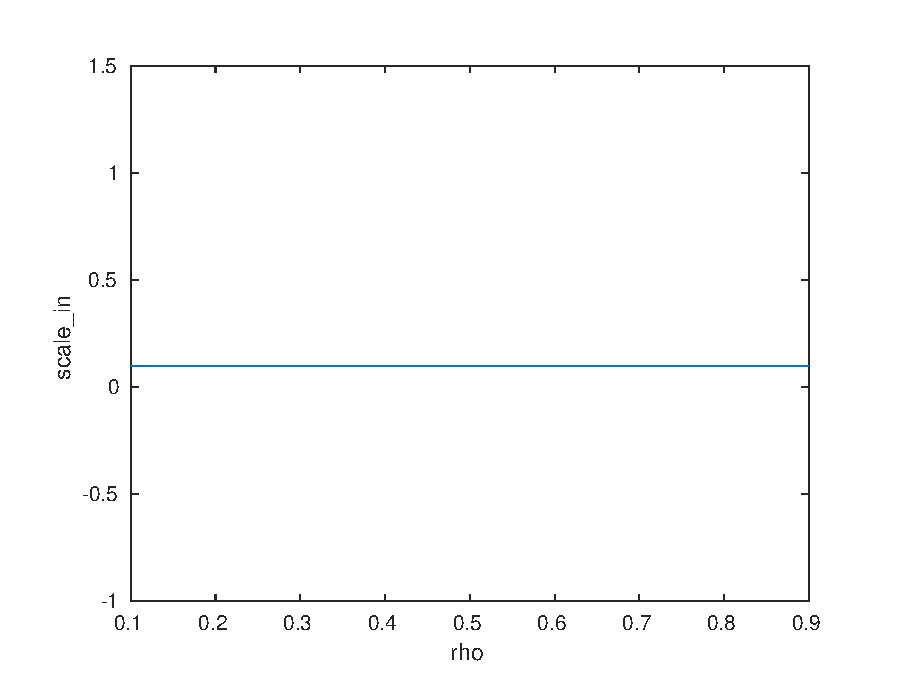
\includegraphics[width=0.6\linewidth]{immagini/scalein}
	\caption{Miglior scelta \textit{input scaling} al variare di rho.}
	\label{fig:scalein}
\end{figure}


Per avere un confronto preciso al livello numerico con il \textit{paper} citato, viene allenta una rete neurale con 500 unità totalmente connessa.
\begin{table}[h]
	\begin{center}
		\begin{tabular}{|c|c|}
			\hline
			Risultati paper & Risultati rete implementata \\
			\hline
			$3.1413 \times 10^{-4} (\pm1.14197 \times 10^{-5}) $ & 
			$3.2159 \times 10^{-4} (\pm1.1701 \times 10^{-5}) $\\
			\hline
		\end{tabular}
	\end{center}
\caption{Error test \textit{ESNtrain()}}
\end{table}

\section{Conclusioni}
I risultati ottenuti con la rete implementata dimostrano il corretto funzionamento di quest'ultima. La rete può dunque essere utilizzata per la computazione di altri \textit{task}, come quelli inseriti nella funzione per la generazione degli stessi. Il modello dunque risulta utile per un primo approccio alle \textit{Echo State Network} e come punto di partenza per la realizzazione di altri modelli. La sua modularità è stata pensata proprio per poter facilitare l'implementazione di reti con configurazioni diverse del \textit{reservoir} per studi futuri.




\begin{thebibliography}{99}
	\bibitem{RCapproch:paper}
Mantas Luko\v{s}evi\v{c}ius, Herbert Jaeger,
Reservoir computing approaches to recurrent neural network training,
Computer Science Review,
Volume 3, Issue 3,
2009,
Pages 127-149.
%ISSN 1574-0137,
%https://doi.org/10.1016/j.cosrev.2009.03.005.
%(http://www.sciencedirect.com/science/article/pii/S1574013709000173).

\bibitem{w} Wolfgang Maass, Thomas Natschläger, Henry Markram,
Real-time computing without stable states: A new frame-
work for neural computation based on perturbations, Neu-
ral Computation 14 (11) (2002) 2531–2560.

\bibitem{h} Herbert Jaeger, The “echo state” approach to analysing
and training recurrent neural networks, Technical Report
GMD Report 148, German National Research Center for
Information Technology, 2001.

\bibitem{Markovianfactor:paper}
Claudio Gallicchio, Alessio Micheli.
Architectural and Markovian factors of echo state networks,
Neural Networks,
Volume 24, Issue 5,
2011,
Pages 440-456.
%ISSN 0893-6080,
%https://doi.org/10.1016/j.neunet.2011.02.002.
%(http://www.sciencedirect.com/science/article/pii/S0893608011000530).

\bibitem{praticalguide}
Lukoševičius M. (2012) A Practical Guide to Applying Echo State Networks. In: Montavon G., Orr G.B., Müller KR. (eds) Neural Networks: Tricks of the Trade. Lecture Notes in Computer Science, vol 7700. Springer, Berlin, Heidelberg.

\bibitem{leakingintegrator}
Herbert Jaeger, Mantas Lukoševičius, Dan Popovici, Udo Siewert,
Optimization and applications of echo state networks with leaky- integrator neurons,
Neural Networks,
Volume 20, Issue 3,
2007,
Pages 335-352,
%ISSN 0893-6080,

%https://doi.org/10.1016/j.neunet.2007.04.016.

%(http://www.sciencedirect.com/science/article/pii/S089360800700041X)


\end{thebibliography}

%%% EVENTUALE
\appendix
\chapter{Codice}
\lstinputlisting[frame=single]{code/setReservoir.m}
\lstinputlisting[frame=single]{code/getTarget.m}
\lstinputlisting[frame=single]{code/train_readout.m}
\lstinputlisting[frame=single]{code/test_readout.m}
\lstinputlisting[frame=single]{code/Tasks.m}
\lstinputlisting[frame=single]{code/istask.m}
\lstinputlisting[frame=single]{code/generateTask.m}
\lstinputlisting[frame=single]{code/ESNtrain.m}
\lstinputlisting[frame=single]{code/ESNtest.m}
\end{document}